\chapter{Sequencing Data}
hard drive with the sequencing data

\paragraph{a biological problem, which sequencing machine is optimal?}
\begin{itemize}
\item (no problem with) repeats
\item read line
\item troughput ($\frac{Millions of reads}{run}$)
\item library preparation compatibility
\item coverage
\item cost: of the sequencing of the machine itself. $\frac{ Reagent cost}{run}$, $\frac{cost}{Mb}$, $\frac{cost}{run}$, service contract
\item accuracy: multipe types of errors: Indel, Substitution, CG deletions (deletions o full CG), A-T bias. The error rate takes in account all the primary errors of the specific instrument.
\item speed / run-time
\item contamination
\end{itemize}


% \begin{figure}[h]
% \caption{Machines for sequencing}\label{balancepancore}
% \centering
% 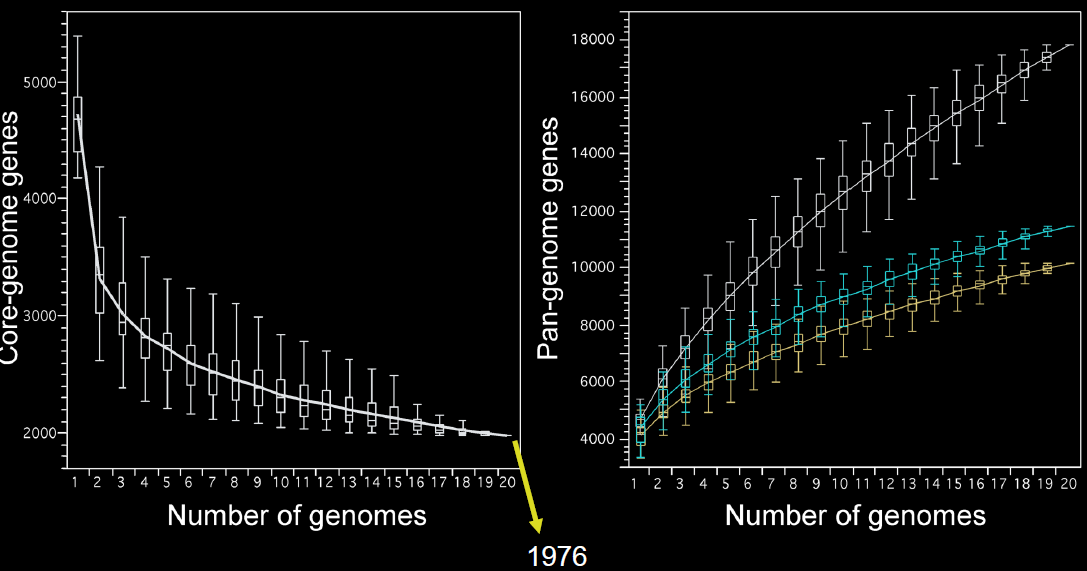
\includegraphics[width=8cm]{corePanGenEcoli}
% \end{figure}


GA II was the first version of illumina. SOLID was a sequencing machine which is not anymore used. Rouche454 responsible of revolution in 2007, not used anymore. MiSeq is also used today. Long read sequencing MinION and pacBio are probably next generation.
pacBio has very log reads and close to single modlecule sequencing.
Ion-Torrent is not anymore used.
MinIon and PacBio gives real time sequencing. 454 quite hifh number of reads but the trouput low.


% \begin{figure}[h]
% \caption{Machines for sequencing}\label{balancepancore}
% \centering
% 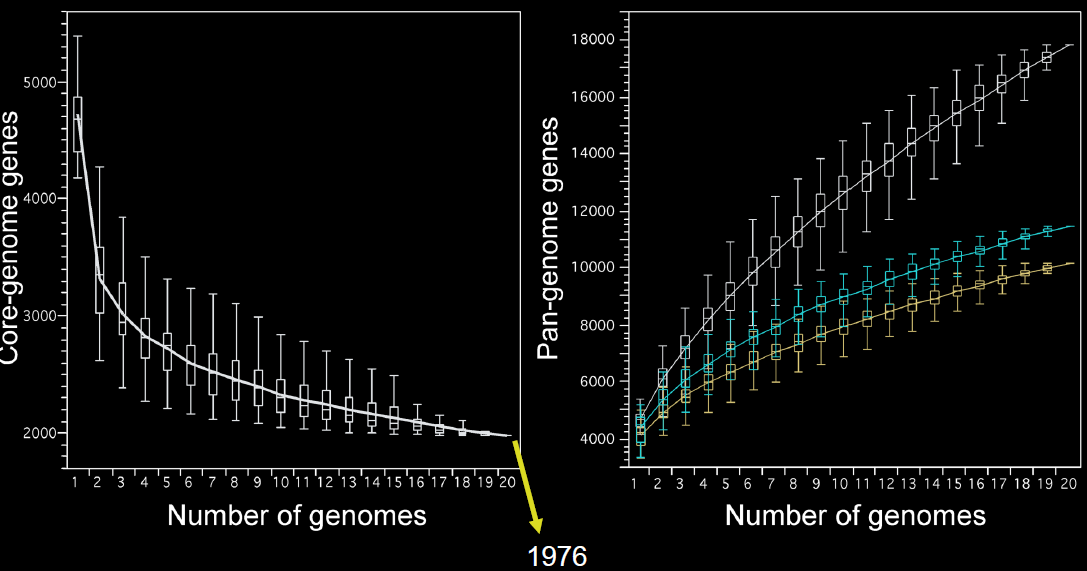
\includegraphics[width=8cm]{corePanGenEcoli}
% \end{figure}


Going towards high throughput.


Illumina NovaSeq is the biggest in the market. very high throughput need.


ILLUMINA has very small machines,  not expensive



% \begin{figure}[h]
% \caption{Machines for sequencing}\label{balancepancore}
% \centering
% 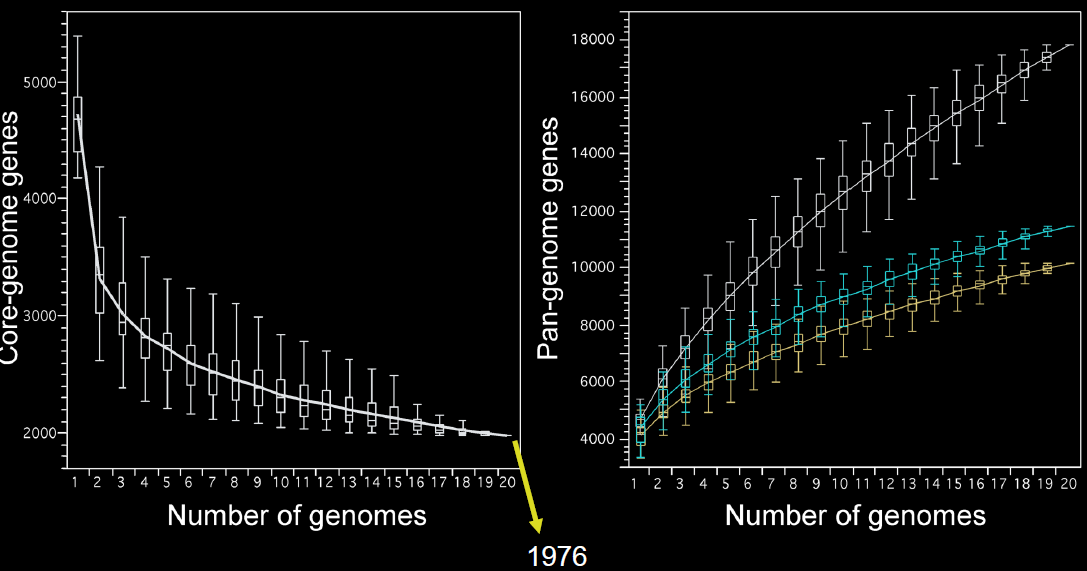
\includegraphics[width=8cm]{corePanGenEcoli}
% \end{figure}


MinION is portable, wet-lab free, real time sequencing. It was used in Ebola pandemic- Used for sequencing DNA, RNA, proteins. The read length follows a Gaussian curve, as there can be also really long reads.


Afer base calling, which is the process through machine converts signals in digits representing the bases. It is made a FASTQ format file. other machines generate other files, but all can at least convert their output in FASTQ. FASTQ contains the sequencing reads and the quality of each base. FASTQ needs to be stored compressed.

Phred- the base calling program, are based on algorithms, to check statistically a sequence.
The phasing noise $\phi$, the intensity scew the intensity of the signal of the closest nucleotide.

siignal decay $\delta$

on ILLUMINA there can be mixed clusters.

Boundary effects: image if zoomed in  it is not really possible to give perimeters to the images of the signals. Overclusteringm akes it very difficult to separate different nucleotide produced signals. Underclustering and Overclustering, optimal clustering in between.



% \begin{figure}[h]
% \caption{Factors to take into account by the base caller}\label{balancepancore}
% \centering
% 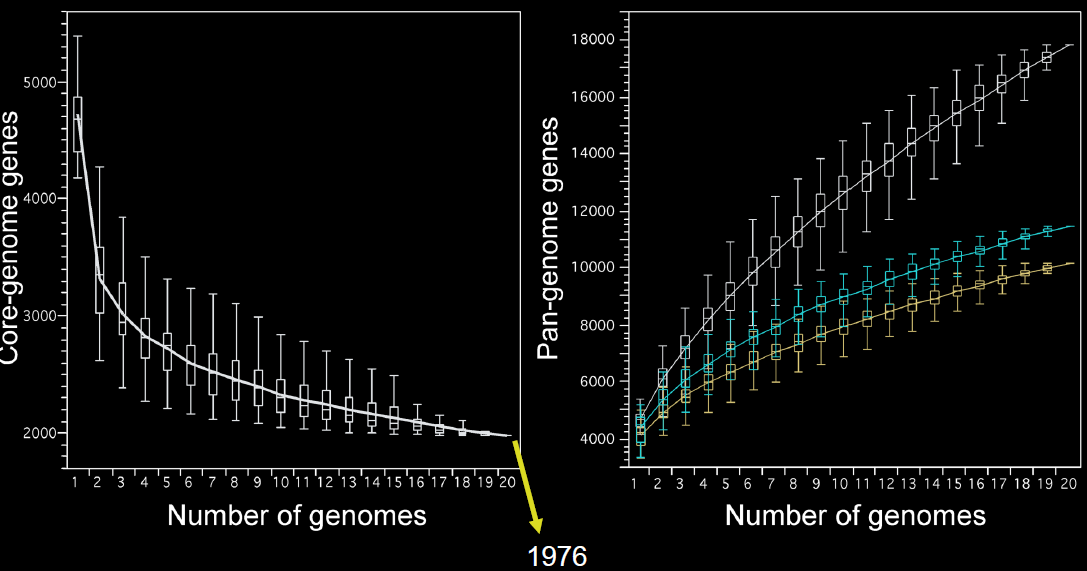
\includegraphics[width=8cm]{corePanGenEcoli}
% \end{figure}



% \begin{figure}[h]
% \caption{Machines for sequencing}\label{balancepancore}
% \centering
% 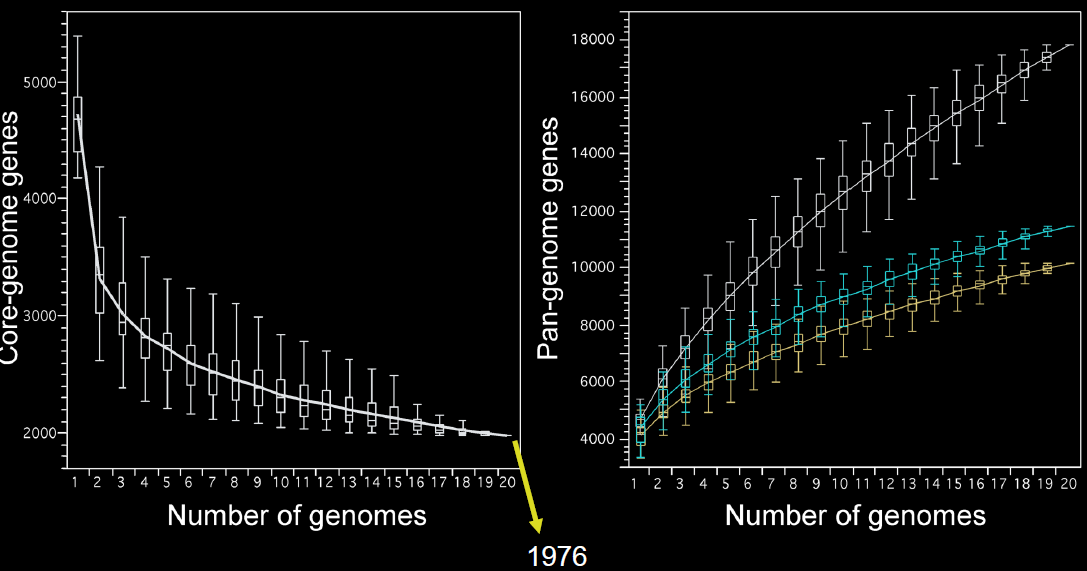
\includegraphics[width=8cm]{corePanGenEcoli}
% \end{figure}


Base-caller has to be performing. By sequencing a known sequence it is possible to evaluate the base caller.

\subsection{FASTQ format}
\begin{enumerate}
\item "@" followed bt a sequence identifier
\item the sequence
\item "+", optionally followd by a sequence identifier
\item The quality scores: several symbols.
\end{enumerate}


\textbf{Base quality:
}
$$ Q = -10 \dot \log_10{p} $$ \text{p = probability of error}

% \begin{figure}[h]
% \caption{Base quality. Going under 0.01$\%$ is quite impossible. 3 to 40} \label{basequal}
% \centering
% \includegraphics[width=8cm]{BaseQuality}
% \end{figure}

Phred+33 transforms integers with characters. Each number can be told in an integer.


% \begin{figure}[h]
% \caption{Base quality. Going under 0.01$\%$ is quite impossible. 3 to 40} \label{basequal}
% \centering
% \includegraphics[width=8cm]{BaseQuality}
% \end{figure}


FASTA format

\begin{enumerate}
\item $">"$ followed by a sequence identifier
\item The sequence
\end{enumerate}


Transform FASTQ in FASTA format file

\subsection{Quality control}
The image under has not a good distribution of read lengths in bp. The first positioned reads are normally the best in terms of quality, Going over the quality lowers. The optimal case would be when quality remains constant. Bugsi n hte base caller could also variate the quality plot. Green, orange and red regions.

Adapters have to be considered to maintain good quality sequences. Removing them means also to reducethe dimension of the output.

$$ x = 1 \text{ciao}$$


Nanopore data maintain the quality of the sequencing.
PacBio seems to behave in really similar way.


\textbf{Distribution of k-mers}: k-mers are a lot in the small numbers region, because of the sequencing errors.


Low-complexity artifacts: low complexity and entropy and high compression.
